The first step of the evaluation was to perform a 10-fold cross-validation in
order to find the decision tree's performance. Using the cross-validation we
found out that the average error of the ten estimates is 10\%. 

Since the predicted subsets has been already calculated from the table examples, the confusion matrix can be easily calculated. To be more specific, the 10 predicted subsets have been concatenated and have been used as input, along with the actual target labels, to the general purpose function which is responsible for the calculation of the confusion matrix.  
The result from the previous step is the matrix below which is the confusion matrix for the 10-fold validation.
See figure~\ref{fig:confusionMatrix}.
\include*{confusion_matrix}

From this matrix it can be easily observed that the correct classification for each
class-emotion are on the matrix's diagonal. So it can been concluded that for the
Surprise there isn't any confusion. On the other hand, for classes there are some misclassified examples. 

For the calculation of the precision and the recall rates per class,two formulas have been used. Those formulas use the information which are already in the confusion matrix and they calculate those two rates.

Those measures are being presented in the table~\ref{fig:averageRecall}
\include*{average_recall_precision}

The figure~\ref{fig:confisionMatixCalc} is an example of a small confusion matrix. It can been used in order to show how the performance measures are beeing calculated.

\begin{figure}[h]
    \centering
    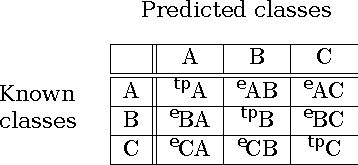
\includegraphics[width=0.3\textwidth]{confusionMatrixCalc.pdf}
    \caption{A simple confusion matrix}
    \label{fig:confisionMatixCalc}
\end{figure}

The recall and the precision can been easily derived from the confusion matrix by applying those formulas:

Precision\textsubscript{A} = tp\textsubscript{A}/(tp\textsubscript{A}+e\textsubscript{BA}+e\textsubscript{CA})

Recall\textsubscript{A} = tp\textsubscript{A}/(tp\textsubscript{A}+e\textsubscript{AB}+e\textsubscript{AC})

The precision and recall rates, along with the F1-measure, reflect our previous conclusions for the classes-emotions.
